\documentclass[a4paper,10pt]{beamer}

\usepackage[utf8]{inputenc}
\usepackage{fontspec}
\usepackage{amsmath}
\usepackage{amssymb}
\usepackage{graphicx}
\usepackage{subcaption}
\usepackage{comment}
\usepackage{wrapfig}
\usepackage{color}
\usepackage{xcolor}
\usepackage{mathtools}
\usepackage{algorithmicx}
\usepackage{algorithm}
\usepackage{algpseudocode}
\usepackage{hyperref}
\usepackage{cleveref}
\usepackage{empheq}

\beamertemplatenavigationsymbolsempty

\usefonttheme{professionalfonts}

\usefonttheme[]{structurebold}

\usetheme{Copenhagen}
\usecolortheme{rose}
\usecolortheme{dolphin}
\useinnertheme{circles}
\useoutertheme{tree}

\addtobeamertemplate{navigation symbols}{}{%
	\usebeamerfont{footline}%
	\usebeamercolor[fg]{footline}%
	\hspace{1em}%
	\insertframenumber/\inserttotalframenumber
}


\setmainfont[Path=/usr/share/fonts/truetype/calibri/,
BoldItalicFont=calibriz.ttf,
BoldFont      =calibrib.ttf,
ItalicFont    =calibrii.ttf]{calibri.ttf}

\newcommand{\BS}[1]{\boldsymbol{#1}}
\newcommand{\E}[1]{\mathbb{E}\left[ #1 \right]}
\newcommand{\sqb}[1]{\left[ #1 \right]}
\newcommand{\rb}[1]{\left( #1 \right)}
\newcommand{\angbrac}[1]{\left \langle #1 \right \rangle}
\newcommand{\norm}[1]{\left| \left| #1 \right| \right|}

\definecolor{burgundy}{RGB}{128,0,32}
\definecolor{darkgreen}{RGB}{4,110,0}

\definecolor{customblue}{rgb}{0.8,0.8,1}
\newcommand*\bluebox[1]{\colorbox{customblue}{\hspace{1em}#1\hspace{1em}}}

\definecolor{custompurple}{RGB}{255,179,179}
\newcommand*\purplebox[1]{\colorbox{custompurple}{\hspace{1em}#1\hspace{1em}}}

\title{Generalized Langevin Equation}
\subtitle{Stochastic Differential Equations}
\author{Sankarasubramanian Ragunathan \newline \newline 389851}
\institute{\textbf{RWTH Aachen University}}
\date{}


\begin{document}
	\begin{frame}
		\titlepage
		\centering
		
\includegraphics[width=0.25\textwidth]{RWTH_Aachen_University_Logo.eps}
	\end{frame}

	\begin{frame}
	\frametitle{Agenda}
		\tableofcontents
	\end{frame}

	\begin{frame}
		\small
		\section{Scope of the Project}
		\frametitle{Scope of the Project}
		
		\begin{itemize}
			\item[What?]{Generalized Langevin Dynamics is a modeling technique that can be used to model anomalous diffusive phenomena observed in viscoelastic fluid flow and in biological systems.}
			
			\item[Why?]{Anomalous diffusion problems: Langevin model fails to capture sub-diffusive and super-diffusive behavior which the GLE succeeds in capturing. But GLE is \textit{Non-Markovian} i.e. \texttt{memory kernel} depends on the history of velocity. This issue is overcome by using Extended Variable GLE that considers a finite dimensional subspace for the \texttt{memory kernel}.}
			
			\item[Where?]{Applications of GLE include but are not restricted to micro-rheology, biological systems, nuclear quantum effects and systems in which anomalous diffusion arise.}
			
			\item[How?]{Study Extended Variable GLE using Prony series approximation. Accuracy of Implicit/Explicit Euler and Splitting Numerical schemes are also tested to find out the optimal scheme. Study the sensitivity of the solution to the changes in the parameters of the extended variable GLE.}
			
		\end{itemize}
	\end{frame}

	\begin{comment}
		\begin{figure}[H]
		\centering
		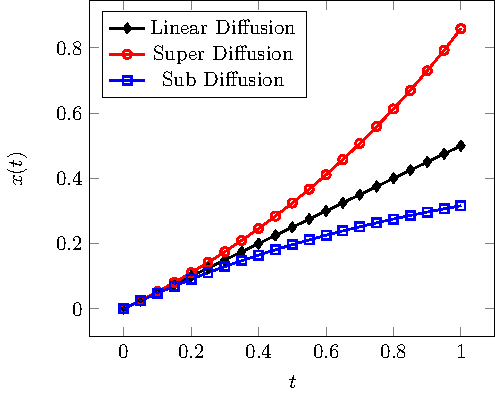
\includegraphics[width=0.35\linewidth]{./Plots/Diffusion.pdf}
		\caption{Anomalous Diffusion: Linear,Sub and Super Diffusive nature}
		\end{figure}
	\end{comment}

	\begin{frame}
		\small
		\section{Introduction to Generalized Langevin Equation}
		\frametitle{Generalized Langevin Equation}
		\subsection{Introduction}
		\framesubtitle{Introduction}
		\begin{itemize}
			\item[What?] {\textbf{Langevin Dynamics:} Large particles in a bath of small particles, motion of large particles directly integrated while the dynamics of small particles are "averaged out".}
			\item[Why?] {\textit{Molecular Dynamics} simulations involving all particles is computationally expensive. Langevin Equation model is computationally cheaper.}
		\end{itemize}
		\begin{minipage}{0.35\linewidth}
			\footnotesize
			\begin{alertblock}{Drawback}
				Anomalous diffusion problems arising due to \textit{Power Law} behavior of solute-solvent systems cannot be solved.
			\end{alertblock}
			\begin{exampleblock}{Solution}
				\textit{Generalized Langevin Equation} (\textbf{GLE})
			\end{exampleblock}
		\end{minipage}
		\hfill
		\begin{minipage}{0.6\linewidth}
			\centering
			\begin{figure}[H]
				\begin{subfigure}[b]{0.45\linewidth}
					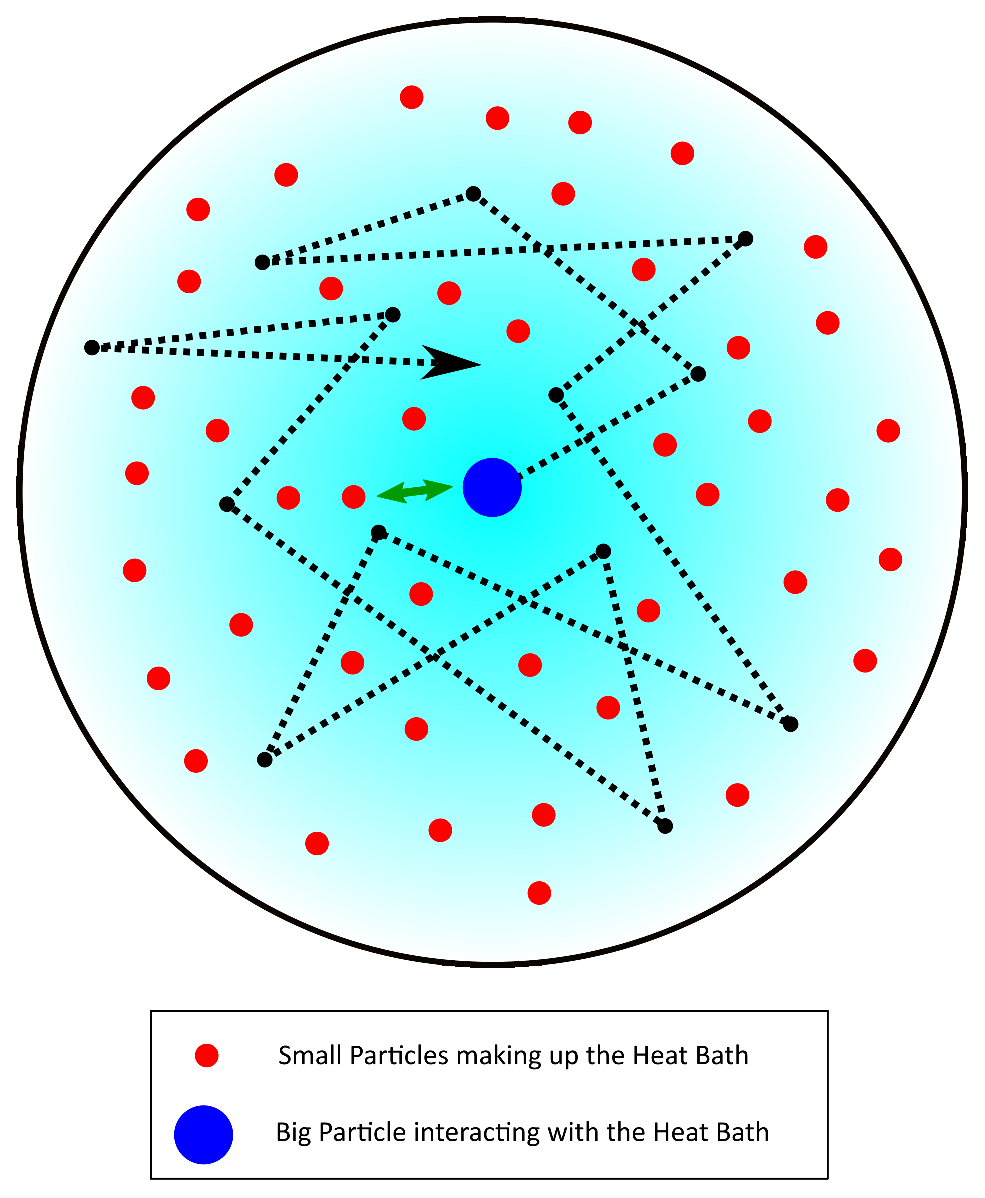
\includegraphics[width=\linewidth]{./Plots/HeatBath.eps}
					\caption{\footnotesize \textcolor{blue}{Big Particles} interacting with \textcolor{red}{Smaller Particles}}
				\end{subfigure}
				\begin{subfigure}[b]{0.5\linewidth}
					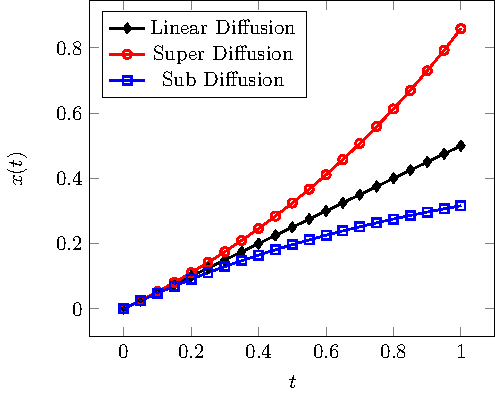
\includegraphics[width=\linewidth]{./Plots/Diffusion.pdf}
					\caption{\footnotesize Sub-diffusive and Super-diffusive behavior of solute-solvent systems}
				\end{subfigure}
			\end{figure}
		\end{minipage}
	\end{frame}		
	
	\begin{frame}
		\small
		\frametitle{Generalized Langevin Equation}
		\subsection{Mathematical Model}
		\framesubtitle{Mathematical Model}
		
		The velocity term of GLE is based on \textit{Ornstein-Uhlenbeck} process.
	
		\begin{block}{GLE Equations}
			\begin{align}
			d\BS{X}(t) &= \BS{V}(t) dt \\
			\BS{M} d\BS{V}(t) &= \underbrace{\vphantom{- \int_{0}^{t} \BS{\Gamma}(t-s) \BS{V}(s) ds dt}\BS{F}^{c}(\BS{X}(t)) dt}_{\text{\centering \begin{minipage}{1.5cm}
					Conservative Force due to Potential
			\end{minipage}}}
			\underbrace{- \int_{0}^{t} \BS{\Gamma}(t-s) \BS{V}(s) ds dt}_{\text{\centering \begin{minipage}{1.5cm}
				Temporally Non-Local Drag Force
				\end{minipage}}\;\rb{\BS{F}^{d}}} + \underbrace{\vphantom{- \int_{0}^{t} \BS{\Gamma}(t-s) \BS{V}(s) ds dt}\BS{F}^{r}(t)dt}_{\text{\begin{minipage}{1.8cm}
				Random Correlated Force given by \textit{FDT}
				\end{minipage}}} \\
			\BS{X}(0) = \BS{X}_{0}, &\qquad \BS{V}(0) = \BS{V}_{0} \qquad (\text{Initial Conditions})
			\end{align}
		\end{block}
		\begin{alertblock}{Note:}
			$\BS{F}^{r}$ and $\BS{F}^{d}$ are characterized by the \texttt{memory kernel} consistent with \textbf{FDT}.
		\end{alertblock}
	\end{frame}

	\begin{frame}
		\small
		\frametitle{Generalized Langevin Equation}
		\framesubtitle{Mathematical Model}
		\begin{theorem}
			FDT (Fluctuation Dissipation Theorem) states that the equilibration to a temperature, $T$, requires that the two-time correlation of $\BS{F}^{r}(t)$ and $\BS{\Gamma}(t)$ be related as:
			\begin{align}
				\angbrac{\BS{F}^{r}_{i}(t+s),\BS{F}^{r}_{j}(t)} = k_{B} T \BS{\Gamma}(s) \delta_{ij}, \qquad s \geq 0
			\end{align}
		\end{theorem}
		where $k_{B}$ is the Boltzmann's Constant and $\delta_{ij}$ is the Kronecker Delta.
		\linebreak
		
		
		\textcolor{red}{\textbf{Note:}}
		\begin{itemize}
			\item {$\BS{F}^{d}(t)$ depends on the velocity history unlike in \textit{Langevin Equation}} where it depends on the velocity at that instant.
			\item {The random forces are not just delta correlated but are correlated by the \texttt{memory kernel}. \textcolor{darkgreen}{\texttt{Memory Kernel} choice and approximation important based on the problem to be studied.}}
		\end{itemize}
	\end{frame}
	
	\begin{frame}
		\frametitle{Generalized Langevin Equation}
		\subsection{Model Complications and Solutions}
		\framesubtitle{Model Complications and Solutions}
		\vspace{-0.8cm}
		\begin{minipage}[t]{0.44\textwidth}
			\begin{alertblock}{\textbf{Complications}}
				\begin{enumerate}
					\item {Storage of subset of the time history of $\BS{V}(t)$.}
					\item {Sequence of $\BS{F}^{r}(t)$ given by \texttt{FDT}.}
					\item {Numerical SDE solution should converge in distribution.}
				\end{enumerate}
			\end{alertblock}
		\end{minipage}
		\hfill
		\begin{minipage}[t]{0.52\textwidth}
			\centering
			\begin{exampleblock}{\textbf{Solution}}
				\begin{enumerate}
					\item {Using extended variable \texttt{Prony Series} for \texttt{Memory Kernel}.
					\scriptsize
					\begin{align}
					 \BS{\Gamma}(t) \approx \sum_{k=1}^{N_{k}} \frac{c_{k}}{\tau_{k}} \exp \sqb{-\frac{t}{\tau_{k}}}, \qquad t \geq 0 \end{align}
					\normalsize
					where $N_{k}$ is the number of terms used in approximating the \texttt{memory kernel}. }
					\item {Using a suitable integration scheme for the numerical method.}
				\end{enumerate}
			\end{exampleblock}
		\end{minipage}
	\end{frame}

	\begin{frame}
		\frametitle{Generalized Langevin Equation}
		\framesubtitle{Model Complications and Solutions}
		\small
		\textcolor{blue}{\textbf{Why use extended variable Prony Series?}}
		
		\begin{itemize}
			\item {Approximation of \texttt{memory kernel} to map {\textbf{Non-Markovian}} GLE to {\textbf{Markovian}} system of $N_{k}$ variables.}
			\item {Typically used for modelling \textit{Power Law} based decay/growth as observed in sub/super diffusive systems.}
		\end{itemize}
		
		\textcolor{blue}{\textbf{Importance of choice of integration scheme?}}
		
		\begin{itemize}
			\item {Conservation of moments of variables of interest such as displacement and velocity (usual variables of interest for MD simulations)}
			\item {Convergence of \textbf{GLE} to Langevin equation in the limit of small $\tau_{k}$ as observed in theory.}
		\end{itemize}
	\end{frame}

	\begin{frame}
		\frametitle{Generalized Langevin Equation}
		\subsection{Extended Variable GLE}
		\framesubtitle{Extended Variable GLE}
		\vspace{-0.3cm}
 		%\textbf{Extended Variable GLE:}
		\tiny
		\begin{block}{Main Extended Variable GLE Equations}
			\vspace{-0.3cm}
			\begin{flalign}
				m_{i} dV_{i}(t) &=  F_{i}^{c}(\BS{X}(t))dt + \sum_{k=1}^{N_{k}} S_{i,k} dt \\
				dX_{i}(t) &= V_{i}(t)dt\\
				dS_{i,k}(t) &= -\frac{1}{\tau_{k}}S_{i,k}(t)dt-\frac{c_{k}}{\tau_{k}}V_{i}(t) dt + \frac{1}{\tau_{k}}\sqrt{2 k_{B} T c_{k}} dW_{i,k}(t)
			\end{flalign}
		\end{block}
		\begin{block}{Auxiliary Extended Variable GLE Equations}
			\vspace{-0.3cm}
			\begin{flalign}
				S_{i,k}(t) &= Z_{i,k}(t) + F_{i,k}(t) \\
				dZ_{i,k}(t) &= -\frac{1}{\tau_{k}} Z_{i,k}(t)dt - \frac{c_{k}}{\tau_{k}}V_{i}(t)dt &&
				Z_{i,k}(t) = -\int_{0}^{t} \frac{c_{k}}{\tau_{k}} \text{exp} \sqb{-\frac{\rb{t-s}}{\tau_{k}}}V_{i}(s)ds \\
				d F_{i, k}(t)&=-\frac{1}{\tau_{k}} F_{i, k}(t) d t +\frac{1}{\tau_{k}} \sqrt{2 {k}_{B} T c_{k}} d W_{i, k}(t) && \angbrac{F_{i,k}(t+s),F_{i,k}(t)} = k_{B}T\frac{c_{k}}{\tau_{k}} \text{exp}\sqb{-\frac{s}{\tau_{k}}} \\
				&\quad && F_{i}^{r}(t) = \sum_{k=1}^{N_{k}} F_{i,k}(t)
			\end{flalign}
		\end{block}
	\end{frame}
	
	\begin{frame}
		\section{Numerical Schemes for Solving GLE}
		\frametitle{Generalized Langevin Equation}
		\subsection{Numerical Schemes}
		\framesubtitle{Numerical Schemes}
		\footnotesize
		\textcolor{blue}{\textbf{Numerical Schemes:}}
		\begin{itemize}
			\item {Explicit Euler Scheme.}
			\item {Splitting Scheme.}
		\end{itemize}
		\begin{alertblock}{Which numerical scheme to choose for solving the problem?}
			{Scheme that is able to conserve the first and second moments of quantities of interest i.e. $\BS{V}(t)$ and $\BS{X}(t)$.}
		\end{alertblock}
		\textcolor{blue}{\textbf{Implementation Details:}}
		\begin{itemize}
			\item {Uniform time-step size, $\Delta t$, where $N_{t} \Delta t = T_{\text{tot}}$ ($T_{\text{tot}}$ represents the total time of the simulation and $N_{t}$ represents the \# of time-steps.)}
			\item {All $N_{p}$ particles are seeded with the same constant $\BS{X}(0)$ and $\BS{V}(0)$ (\textcolor{red}{\textbf{Note:}} We could also seed the initial conditions based on the p.d.f if known.)}
			\item {The composite variable $S_{i,k}(t)$ is assumed to be zero initially.}
		\end{itemize}
	\end{frame}

\begin{comment}
	\begin{frame}
		\frametitle{Generalized Langevin Equation}
		\framesubtitle{Numerical Schemes}
		\textcolor{blue}{\textbf{Implementation Details:}}
		\begin{itemize}
			\item {Uniform time-step size, $\Delta t$, where $N_{t} \Delta t = T_{\text{tot}}$ ($T_{\text{tot}}$ represents the total time of the simulation and $N_{t}$ represents the \# of time-steps.)}
			\item {All $N_{p}$ particles are seeded with the same constant $\BS{X}(0)$ and $\BS{V}(0)$ (\textcolor{red}{\textbf{Note:}} We could also seed the initial conditions based on the p.d.f if known.)}
			\item {The composite variable $S_{i,k}(t)$ is assumed to be zero initially.}
		\end{itemize}
	\end{frame}
\end{comment}
	
	\begin{frame}
		\frametitle{Generalized Langevin Equation}
		\framesubtitle{Numerical Schemes}
			\vspace{-0.3cm}
			\begin{algorithm}[H]
				\scriptsize
				\renewcommand{\algorithmicrequire}{\textbf{Input:}}
				\renewcommand{\algorithmicensure}{\textbf{Output:}}
				\begin{algorithmic}[1]
					\Require $\BS{X}(0)$,$\BS{V}(0)$,$\BS{S}(0)$
					\Ensure $\BS{X}(t)$,$\BS{V}(t)$
					\For{$n=0$ to $N_{t}$}
					\tiny
						\State $V_{i}^{n+1} = V_{i}^{n} + \frac{\Delta t}{m_{i}} F_{i}^{c} \rb{\BS{X}^{n}}+\frac{\Delta t}{m_{i}} \sum_{k=1}^{N_{k}}S_{i,k}^{n}$
						\Comment Advance $\BS{V}(t)$ by a full step
						\State $X_{i}^{n+1} = X_{i}^{n} + \Delta t V_{i}^{n}$
						\Comment Advance $\BS{X}(t)$ by a full step
						\State $S_{i,k}^{n+1} = \rb{1-\frac{\Delta t}{\tau_{k}}}S_{i,k}^{n}-\frac{c_{k}\Delta t}{\tau_{k}}V_{i}^{n} + \frac{1}{\tau_{k}}\sqrt{2 k_{B} T c_{k}}\Delta W_{i,k}$
						\Comment Advance $\BS{S}(t)$ by a full step
					\scriptsize
					\EndFor
				\end{algorithmic}
				\caption*{\footnotesize Explicit Euler Scheme}
			\end{algorithm}
			\vspace{-0.75cm}
			\begin{algorithm}[H]
				\scriptsize
				\renewcommand{\algorithmicrequire}{\textbf{Input:}}
				\renewcommand{\algorithmicensure}{\textbf{Output:}}
				\begin{algorithmic}[1]
					\Require $\BS{X}(0)$,$\BS{V}(0)$,$\BS{S}(0)$
					\Ensure $\BS{X}(t)$,$\BS{V}(t)$
					\For{$n=0$ to $N_{t}$}
					\tiny
					\State $V_{i}^{n+1/2} = V_{i}^{n} + \frac{\Delta t}{2m_{i}} F_{i}^{c} \rb{\BS{X}^{n}}+\frac{\Delta t}{2m_{i}} \sum_{k=1}^{N_{k}}S_{i,k}^{n}$
					\Comment Advance $\BS{V}(t)$ by a half step
					\State $X_{i}^{n+1} = X_{i}^{n} + \Delta t V_{i}^{n+1/2}$
					\Comment Advance $\BS{X}(t)$ by a full step
					\State $S_{i,k}^{n+1} = \theta_{k} S_{i,k}^{n}-\rb{1-\theta_{k}}c_{k}V_{i}^{n+1/2} + \alpha_{k}\sqrt{2 k_{B} T c_{k}}\Delta W_{i,k}$
					\Comment Advance $\BS{S}(t)$ by a full step
					\State $V_{i}^{n+1} = V_{i}^{n+1/2} + \frac{\Delta t}{2m_{i}} F_{i}^{c} \rb{\BS{X}^{n+1}}+\frac{\Delta t}{2m_{i}} \sum_{k=1}^{N_{k}}S_{i,k}^{n+1}$
					\Comment Advance $\BS{V}(t)$ by a half step
					\scriptsize
					\EndFor
				\end{algorithmic}
				\caption*{\footnotesize Splitting Scheme}
			\end{algorithm}
	\end{frame}

	\begin{frame}
		\frametitle{Generalized Langevin Equation}
		\subsection{Comparison of Numerical Schemes}
		\framesubtitle{Comparison of Numerical Schemes}
		\textcolor{blue}{\textbf{Case Study:}}
		\begin{itemize}
			\item {One dimensional problem, $d = 1$}
			\item {Single mode in the Prony series approximation, $N_{k} = 1$}
			\item {Zero conservative force acting on the particles, $\BS{F}^{c}\rb{\BS{X}(t)} = 0$}
		\end{itemize}
		The case study is simulated using both numerical schemes, \textit{Explicit Euler} and \textit{Splitting Method}, for three different $\tau$ and $c$ values in the \texttt{Prony Series} approximation (\Cref{tab:cTauBaseCase})
		\begin{table}[H]
			\begin{tabular}{| p{2.6cm} | c | c |}
				\hline
				\textbf{Type of System} & $\BS{c}$ & $\BS{\tau}$ \\
				\hline
				Under-damped & 1 & 1 \\
				Critically-damped & 0.5 & 0.5 \\
				Over-damped & 0.25 & 0.25 \\
				\hline
			\end{tabular}
			\caption{$c$ and $\tau$ values used for the case study}
			\label{tab:cTauBaseCase}
		\end{table}
	\end{frame}

	\begin{frame}
		\footnotesize
		\frametitle{Generalized Langevin Equation}
		\framesubtitle{Comparison of Numerical Schemes - Results}
		\begin{figure}[H]
			\centering
			\begin{subfigure}[b]{0.326\linewidth}
				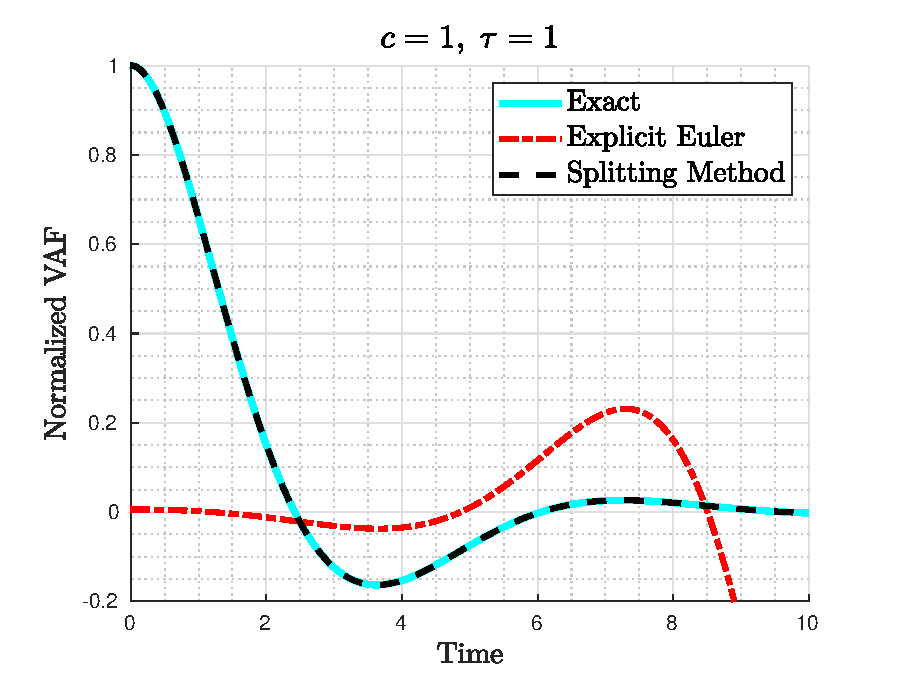
\includegraphics[width=\linewidth]{./Plots/CaseStudy/Underdamped.eps}
				\caption{Under-damped}
			\end{subfigure}
			\begin{subfigure}[b]{0.326\linewidth}
				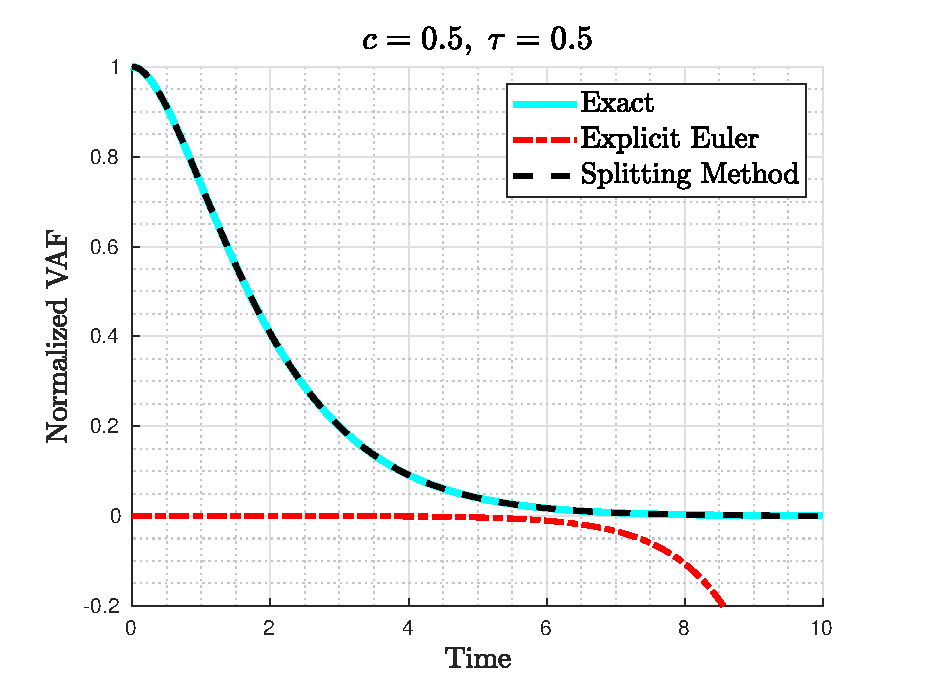
\includegraphics[width=\linewidth]{./Plots/CaseStudy/Criticallydamped.eps}
				\caption{Critically-damped}
			\end{subfigure}
			\begin{subfigure}[b]{0.326\linewidth}
				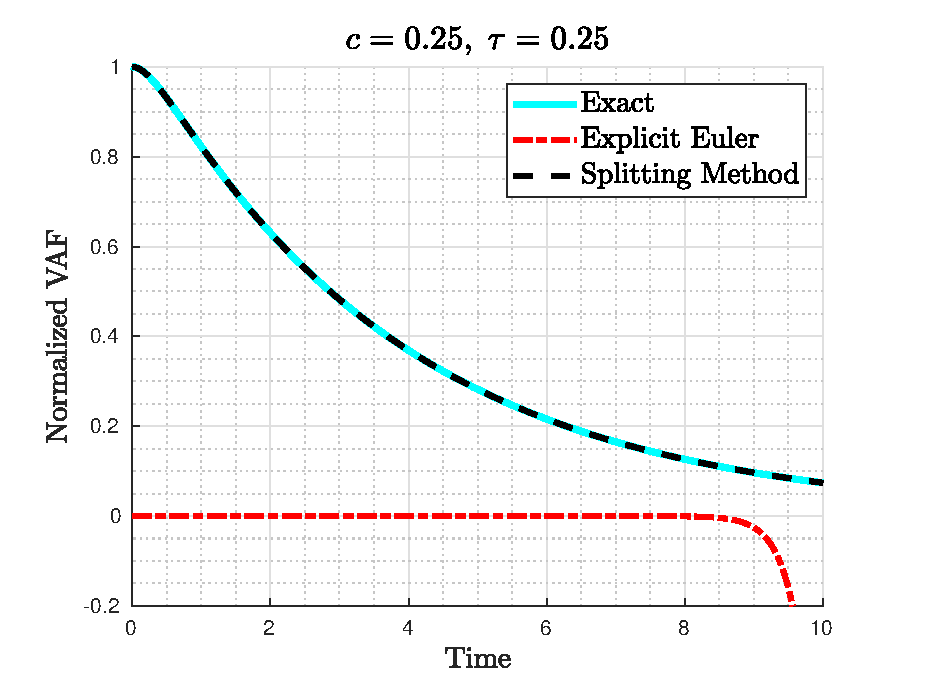
\includegraphics[width=\linewidth]{./Plots/CaseStudy/Overdamped.eps}
				\caption{Over-damped}
			\end{subfigure}
			\caption{Comparison of different numerical schemes w.r.t. Normalized VAF}
		\end{figure}
		\vspace{-0.5cm}
		\begin{alertblock}{Normalized VAF (\textit{Velocity Autocorrelation Function})}
			\begin{align}
				\frac{\angbrac{\BS{V}(t),\BS{V}(0)}}{\angbrac{\BS{V}(0),\BS{V}(0)}} = 
				\begin{cases}
				\text{exp} \sqb{-\frac{t}{2 \tau}} \rb{\cos\rb{\Omega t} + \frac{1}{2\tau\Omega} \sin\rb{\Omega t}}  &\text{for} \; \Omega \neq 0 \\
				\text{exp} \sqb{-\frac{t}{2 \tau}} \rb{1 + \frac{t}{2 \tau}} &\text{for} \; \Omega = 0
				\end{cases}
			\end{align}
			\begin{gather}
				\notag
				\Omega = \sqrt{c/\tau - 1/4\tau^{2}}
			\end{gather}
		\end{alertblock}
	\end{frame}
	\begin{frame}
		\frametitle{Generalized Langevin Equation}
		\framesubtitle{Comparison of Numerical Schemes - Results}
		\large
		\textcolor{blue}{\textbf{Observation:}}
		{Explicit Euler scheme produces wrong results for the \texttt{Normalized VAF} as when compared to the Splitting scheme.} \\
		\vspace{0.25cm}
		\textcolor{blue}{\textbf{Solution:}}
		{Using the Splitting scheme as the preferred integration scheme for all proceeding cases.}
	\end{frame}
	
	\begin{frame}
		\frametitle{Generalized Langevin Equation}
		\subsection{Harmonic Potential Well}
		\framesubtitle{Harmonic Potential Well}
		\begin{block}{Harmonic Potential Well GLE}
			\footnotesize
			\begin{align}
				d\BS{V}(t) = \underbrace{\vphantom{\int_{0}^{t} \frac{\gamma_{\lambda}}{\Gamma_{0} \rb{1-\lambda}}\rb{t-s}^{-\lambda} \BS{V}(s) ds dt} -\omega^{2}_{0} \BS{X}(t)}_{\text{\begin{minipage}{0.165\linewidth}
						Conservative Force arising from Harmonic Potential
						\end{minipage}}}dt - \underbrace{\int_{0}^{t} \frac{\gamma_{\lambda}}{\Gamma_{0} \rb{1-\lambda}}\rb{t-s}^{-\lambda}}_{\text{\begin{minipage}{0.165\linewidth}
						\textit{Power Law} decay \texttt{memory kernel} function
						\end{minipage}}} \BS{V}(s) ds dt + \BS{M}^{-1} \BS{F}^{r}(t) dt
						\label{eq:HarmonicGLE}
			\end{align}
		\end{block}
		\textcolor{blue}{\textbf{Question?}} \\ Approximation of the \texttt{memory kernel} in \Cref{eq:HarmonicGLE} using Prony series \\
		\textcolor{blue}{\textbf{Answer:}} \\
		\textit{log}-spaced values for $\tau_{k}$ from $\Delta t/10$ to $10N_{t}\Delta t$ and then linearly fitting $c_{k}$ i.e. $\min_{\BS{x}} \norm{\BS{A}\cdot \BS{x}-\BS{b}}^{2}, \quad \BS{x} = \left\{ c_{k} \right\} \quad \forall k=1, \cdots, N_{k}$
	\end{frame}

	\begin{frame}
		\frametitle{Generalized Langevin Equation}
		\framesubtitle{Harmonic Potential Well - Parameter Fitting}
		\begin{figure}[H]
			\centering
			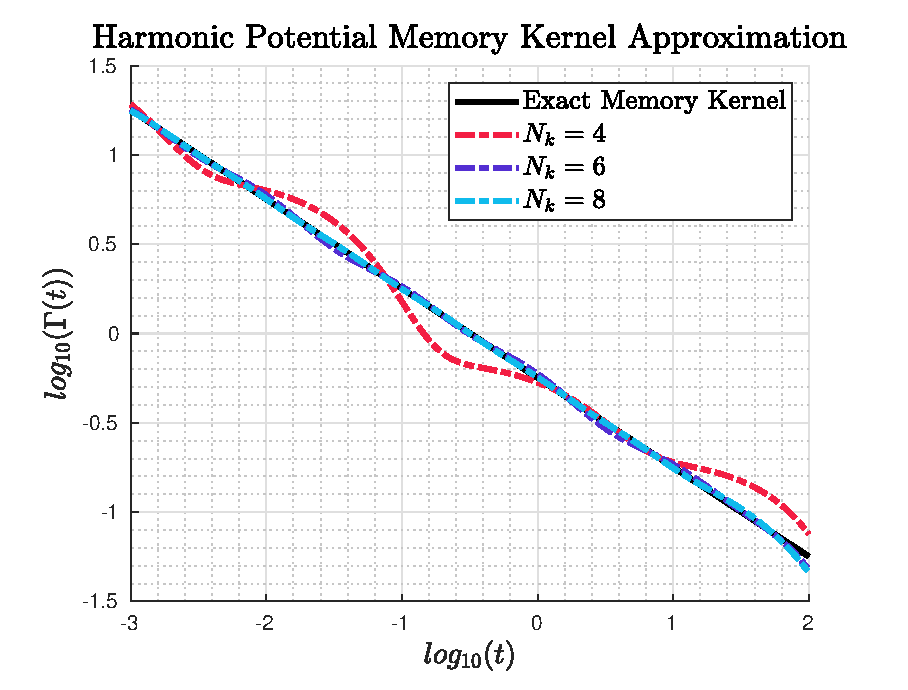
\includegraphics[width=0.725\linewidth]{./Plots/ParameterFittingExample/paramFit.eps}
			\caption{A Prony series fit of the \textit{power law} memory kernel in \cref{eq:HarmonicGLE} for
				$\gamma_{\lambda} = 1$, $\lambda = 0.5$ for different $N_{k}$}
		\end{figure}
	\end{frame}
\end{document}